\section*{OSN 16 Информационная безопасность. Шифрование данных. Криптографическая стойкость. Симметричная криптография. Блочный шифр (DES) и его режимы. Ассиметричные схемы (RSA и Диффи-Хеллмана). Код аутентификации (MAC). Цифровая подпись(DSA).}

\subsubsection{Информационная безопасность, шифрование данных}

\textbf{Безопасность информации (данных)} -- состояние защищенности информации (данных), при котором обеспечены ее (их) \textit{конфиденциальность, целостность и доступность}.

\textbf{Конфиденциальность}: обеспечение доступа к информации только авторизованным пользователям.

\textbf{Целостность}: обеспечение достоверности и полноты информации и методов её обработки.

\textbf{Доступность}: обеспечение доступа к информации и связанным с ней активам авторизованных пользователей по мере необходимости.

\textbf{Криптография} -- наука о методах обеспечения конфиденциальности, целостности данных, аутентификации, невозможности отказа от авторства.

\textbf{Шифрование} -- обратимое преобразование открытого (исходного) текста на основе секретного алгоритма или ключа в шифрованный текст.

\textbf{Прицнип Керкгоффса, максима Шеннона} -- алгоритмы шифрования общедоступны, секретны только ключи.

\subsubsection{Криптографическая стойкость}

\textbf{Криптографическая стойкость} -- способность криптографического алгоритма противостоять криптоанализу.

\textbf{Абсолютно стойкие системы} -- криптосистема не может быть раскрыта (дешифрована) ни теоретически, ни практически даже при наличии у атакующего бесконечно больших вычислительных ресурсов.

\textbf{Достаточно стойкие системы} -- потенциальная возможность дешифрования существует (обратное не доказано), оценка стойкости выполняется в расчёте на определенный момент времени последовательно с двух позиций: вычислительная сложность полного перебора и известные на данный момент слабости (уязвимости) криптосистемы и их влияние на вычислительную сложность -- доказуемая стойкость.

Доказательство стойкости криптосистемы сводится к решению определенной трудно решаемой математической проблемы, положенной в основу алгоритма.

\subsubsection{Симметричная криптография. Блочный шифр (DES) и его режимы}

\textbf{DES (Data Encryption Standard} -- блочный, симметричный шифр. Разработан в январе 1977. Размер блока: 64 бит, размер ключа: 56 бит.

Шифрование одного блока: начальная перестановка, 16 циклов шифрования, конечная (обратная) перестановка.

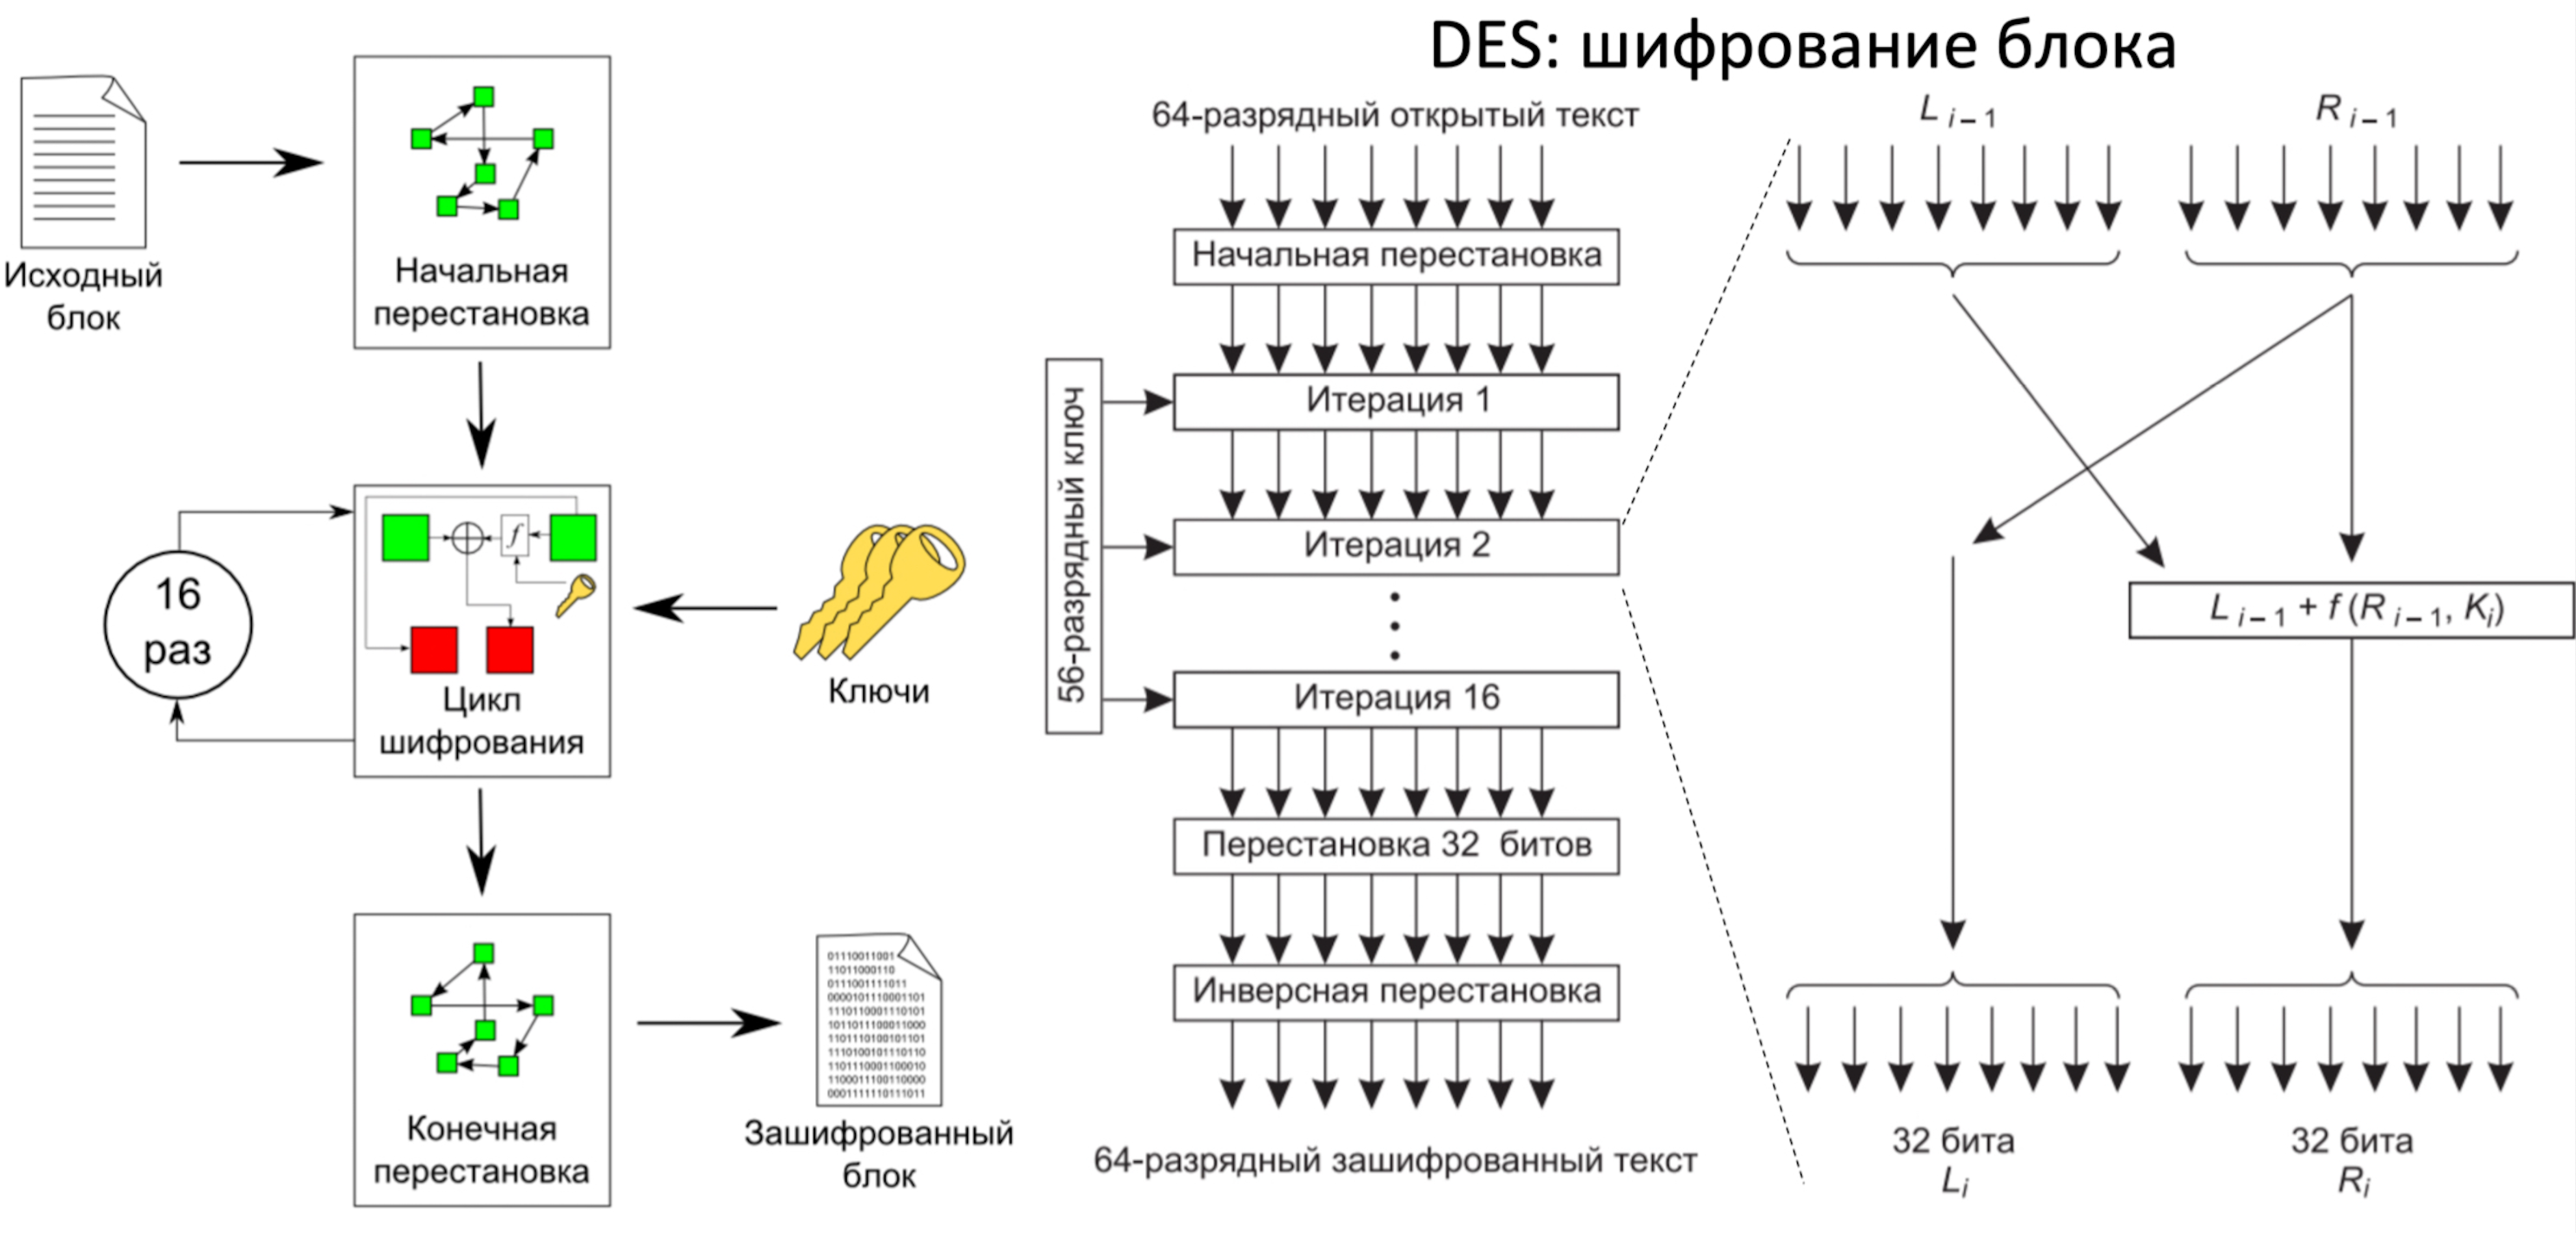
\includegraphics[width=\linewidth]{pics/DES.png}

\begin{wrapfigure}[9]{r}{0.3\linewidth}
\vspace{-4.5ex}
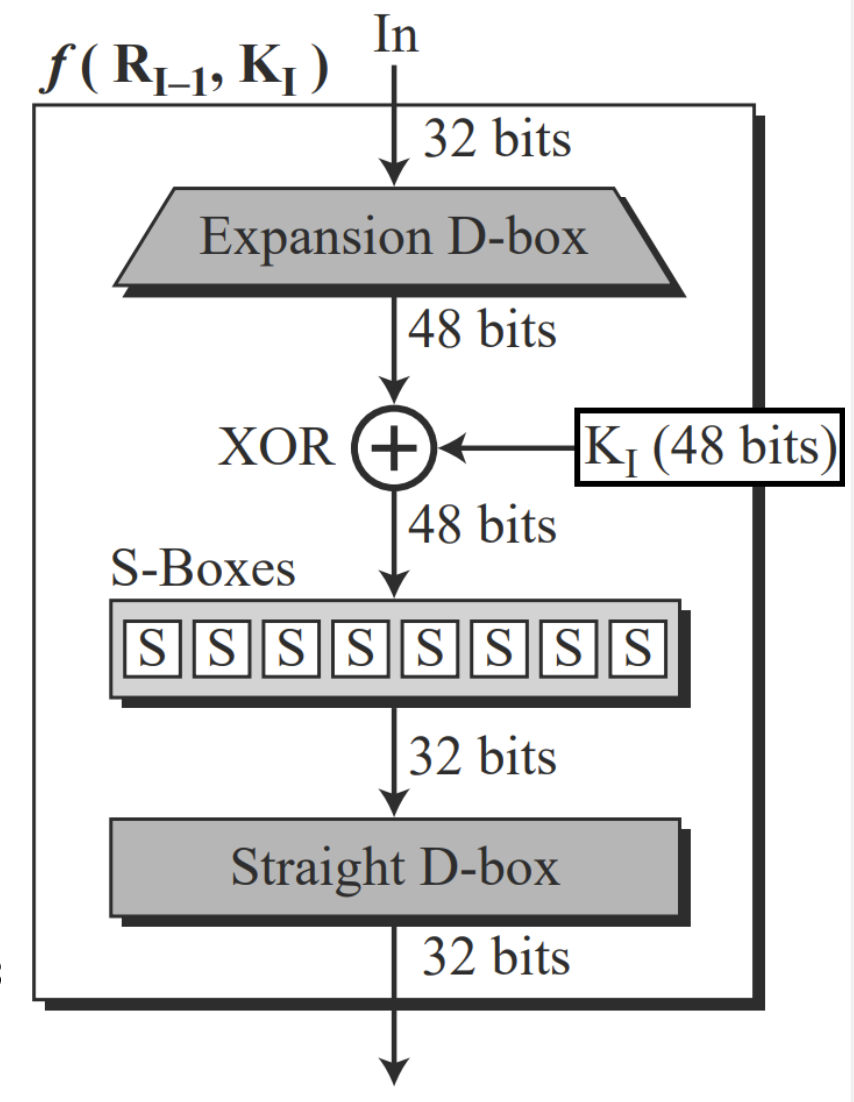
\includegraphics[scale=0.2]{pics/DES_cipher.png}
\end{wrapfigure}

\textbf{DES: функция шифрования $f$}

\begin{itemize}
    \item Функция расширения $E(R_{i-1})$ -- расширяет вектор размером 32 бит до 48 бит путем повторения некоторых бит
    \item Побитовое сложение по модулю 2 расширенного вектора $E(R_{i-1})$ с ключом этого цикла $K_i$. Исходный ключ (56 бит) $\rightarrow$ 16 ключей, каждый по 48 бит, по одному ключу на итерацию. Результат сложения: $B_1B_2B_3B_4B_5B_6B_7B_8$
\end{itemize}

\begin{itemize}
    \item Преобразование $S$ (48 бит $\rightarrow$ 32 бит).
    $B_1B_2B_3B_4B_5B_6B_7B_8$ $\rightarrow$ $B'_1B'_2B'_3B'_4B'_5B'_6B'_7B'_8$.
    $B_i$ (6 бит) $\rightarrow$ $B'_i$ (4 бит), $i = 1..8$
    \item Перестановка $P$
\end{itemize}

\textbf{Тройное шифрование DES (Triple DES)}

Два ключа ($K_1, K_2$), три этапа ($E, D, E$). Ключа длиной 112 бит ($= 2 * 56$) вполне достаточно. Обратная совместимость с существующими DES системами с одним ключом ($K_1 = K_2$).

\subsubsection{Ассиметричные схемы (RSA и Диффи-Хеллмана)}

\textbf{Схема RSA} -- основана на трудоемкости задачи факторизации (разложения на множители) произведения двух простых чисел. Для обеспечения достаточного уровня защищенности требуется ключ длиной, по крайней мере, 1024 бита. Схема слишком медленная, чтобы шифровать большие объемы данных – широко применяется для распространения ключей.

\begin{enumerate}
    \item Выбирается дву различных больших простых числа $p$ и $q$ (обычно 1024 бита)
    \item Вычисляется: $n = p*q$, $(p - 1)(q - 1) = \varphi(n)$
    \item Выбирается число $e$ -- открытая экспонента, взаимно простое с числом $\varphi(n)$
    \item Вычисляется $d = e^{-1} \mod \varphi(n)$
\end{enumerate}

Для сообщения $0 \leq m \leq n - 1$:

\textit{Шифрование}: $c = m^e(\mod n)$, $(e, n)$ -- закрытый ключ

\textit{Дешифрование} (используется теорема Эйлера): $m = c^d(\mod n)$, $d$ - закрытый ключ

\textbf{Протокол Диффи-Хеллмана} -- позволяет двум и более сторонам получить общий секретный ключ, используя не защищенный от прослушивания канал связи. Основан на трудоемкости задачи вычисления дискретного логарифма: обращение функции $g^x$ в некоторой конечной мультипликативной группе $G$.

\begin{wrapfigure}[7]{l}{0.45\linewidth}
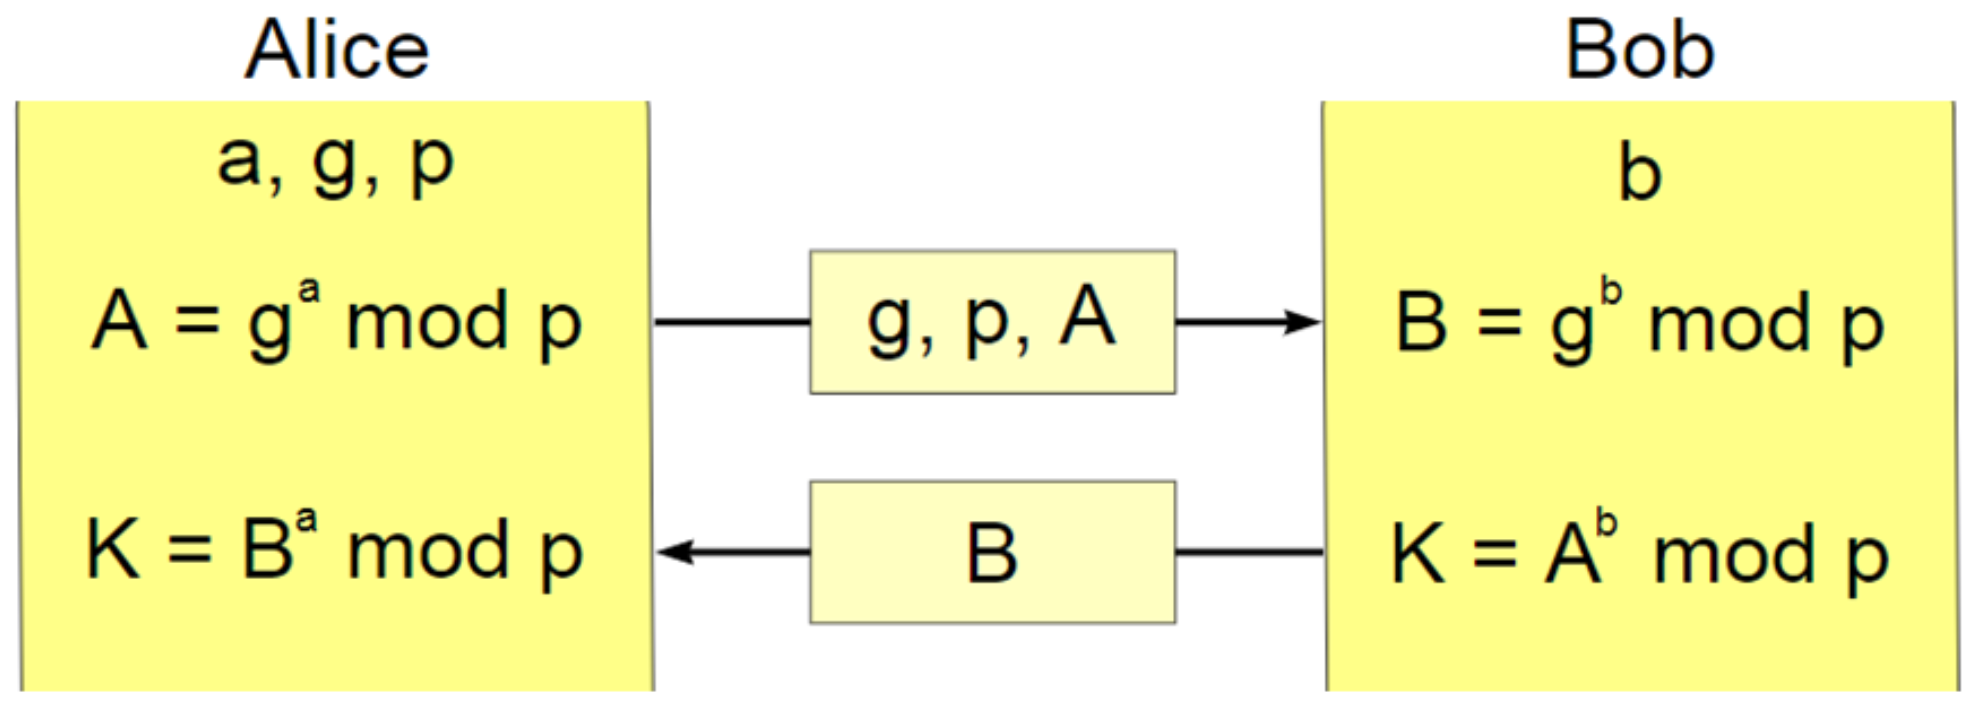
\includegraphics[width=\linewidth]{pics/diffi-hellman.png}
\end{wrapfigure}

\textbf{$a, b$} -- натуральные числа, закрытые ключи

\textbf{$p$} -- случайное число

\textbf{$g$} -- первообразный корень по модулю $p$. Образующий элемент мультипликативной группы кольца вычетов по модулю $p$ $\implies$ $g$ и $p$ взаимно просты

\subsubsection{Код аутентификации (MAC)}

Используя все биты сообщения, отправитель генерирует избыточный код (дополнение) и передает его вместе с сообщением.
Прежде чем принять сообщение как подлинное, получатель выполняет проверку: содержимое сообщения и его дополнение являются согласованными.
Дополнение называется кодом аутентификации сообщения: MAC – Message Authentication Code. Задачи MAC:

\textit{Целостность сообщения} -- в процессе передачи не было непреднамеренной модификации сообщения

\textit{Подлинность сообщения} -- в процессе передачи не было преднамеренной модификации сообщения

\subsubsection{Цифровая подпись(DSA)}

Аналог <<рукописной подписи>> для цифровых документов.

Требования:
\begin{enumerate}
    \item получатель может проверить объявленную личность 
    \item отправитель не может позднее отрицать содержимое сообщения
    \item получатель не может позднее изменить подписанное сообщение
\end{enumerate}

\textbf{Общие параметры схемы:}

$H(x)$ -- криптографическая хэш-функция

$L, N$ -- длина открытого и закрытого ключей

$q$ -- простое число длиной $N$ бит

$p$ -- простое число длиной L бит такое, что $p - 1$ делится на $q$

$h \in (1, p - 1)$ -- произвольное число

$g = h^{\frac{p-1}{q}}(\mod p), q \neq 1$

Параметры схемы для \textbf{каждого пользователя}:

Закрытый ключ $x$ -- случайно выбранное число: $0 < x < q$

Открытый ключ $y = g^x(\mod p)$

\textbf{Генерация подписи сообщения}:

1. Для каждого сообщения $m$ выбирается случайное число k: $1 < k < q$

2. $r = (g^k \mod p) \mod q$. Если $r = 0$, вернуться на шаг 1 и выбрать новое случайное число $k$

3. $s = k^{-1}(H(m) + x * r) \mod q$. Если $s = 0$, вернуться на шаг 1 и выбрать новое случайное число $k$

4. Цифровая подпись: $(r, s)$

\textbf{Проверка подписи}: подпись заведомо неверна, если не выполнено хотя бы одно из условий $0 < r < q, 0 < s < q$. Далее:

1. $w = s^{-1} \mod q$

2. $u_1 = H(m) * w \mod q$

3. $u_2 = r * w \mod q$

4. $v = (g^{u_1}y^{u_2} \mod p) \mod q$

5. Цифровая подпись $(r, s)$ верна $\Leftrightarrow$ $v = r$